\section{Operating Basics}

\subsection{Introduction}

To ensure a good understanding of controllers and controlling theory, a laboratory experiment was performed. As the plant, a motor was used whose speed had to be controlled.
The step function was measured and analyzed at first. Knowing the step function it was very easy to implement a suitable PID controller.

\subsection{Step Function}

To determine the characteristics of the system, a step is applied to the input. Then the output is observed.

\begin{figure}[H]
\begin{center}
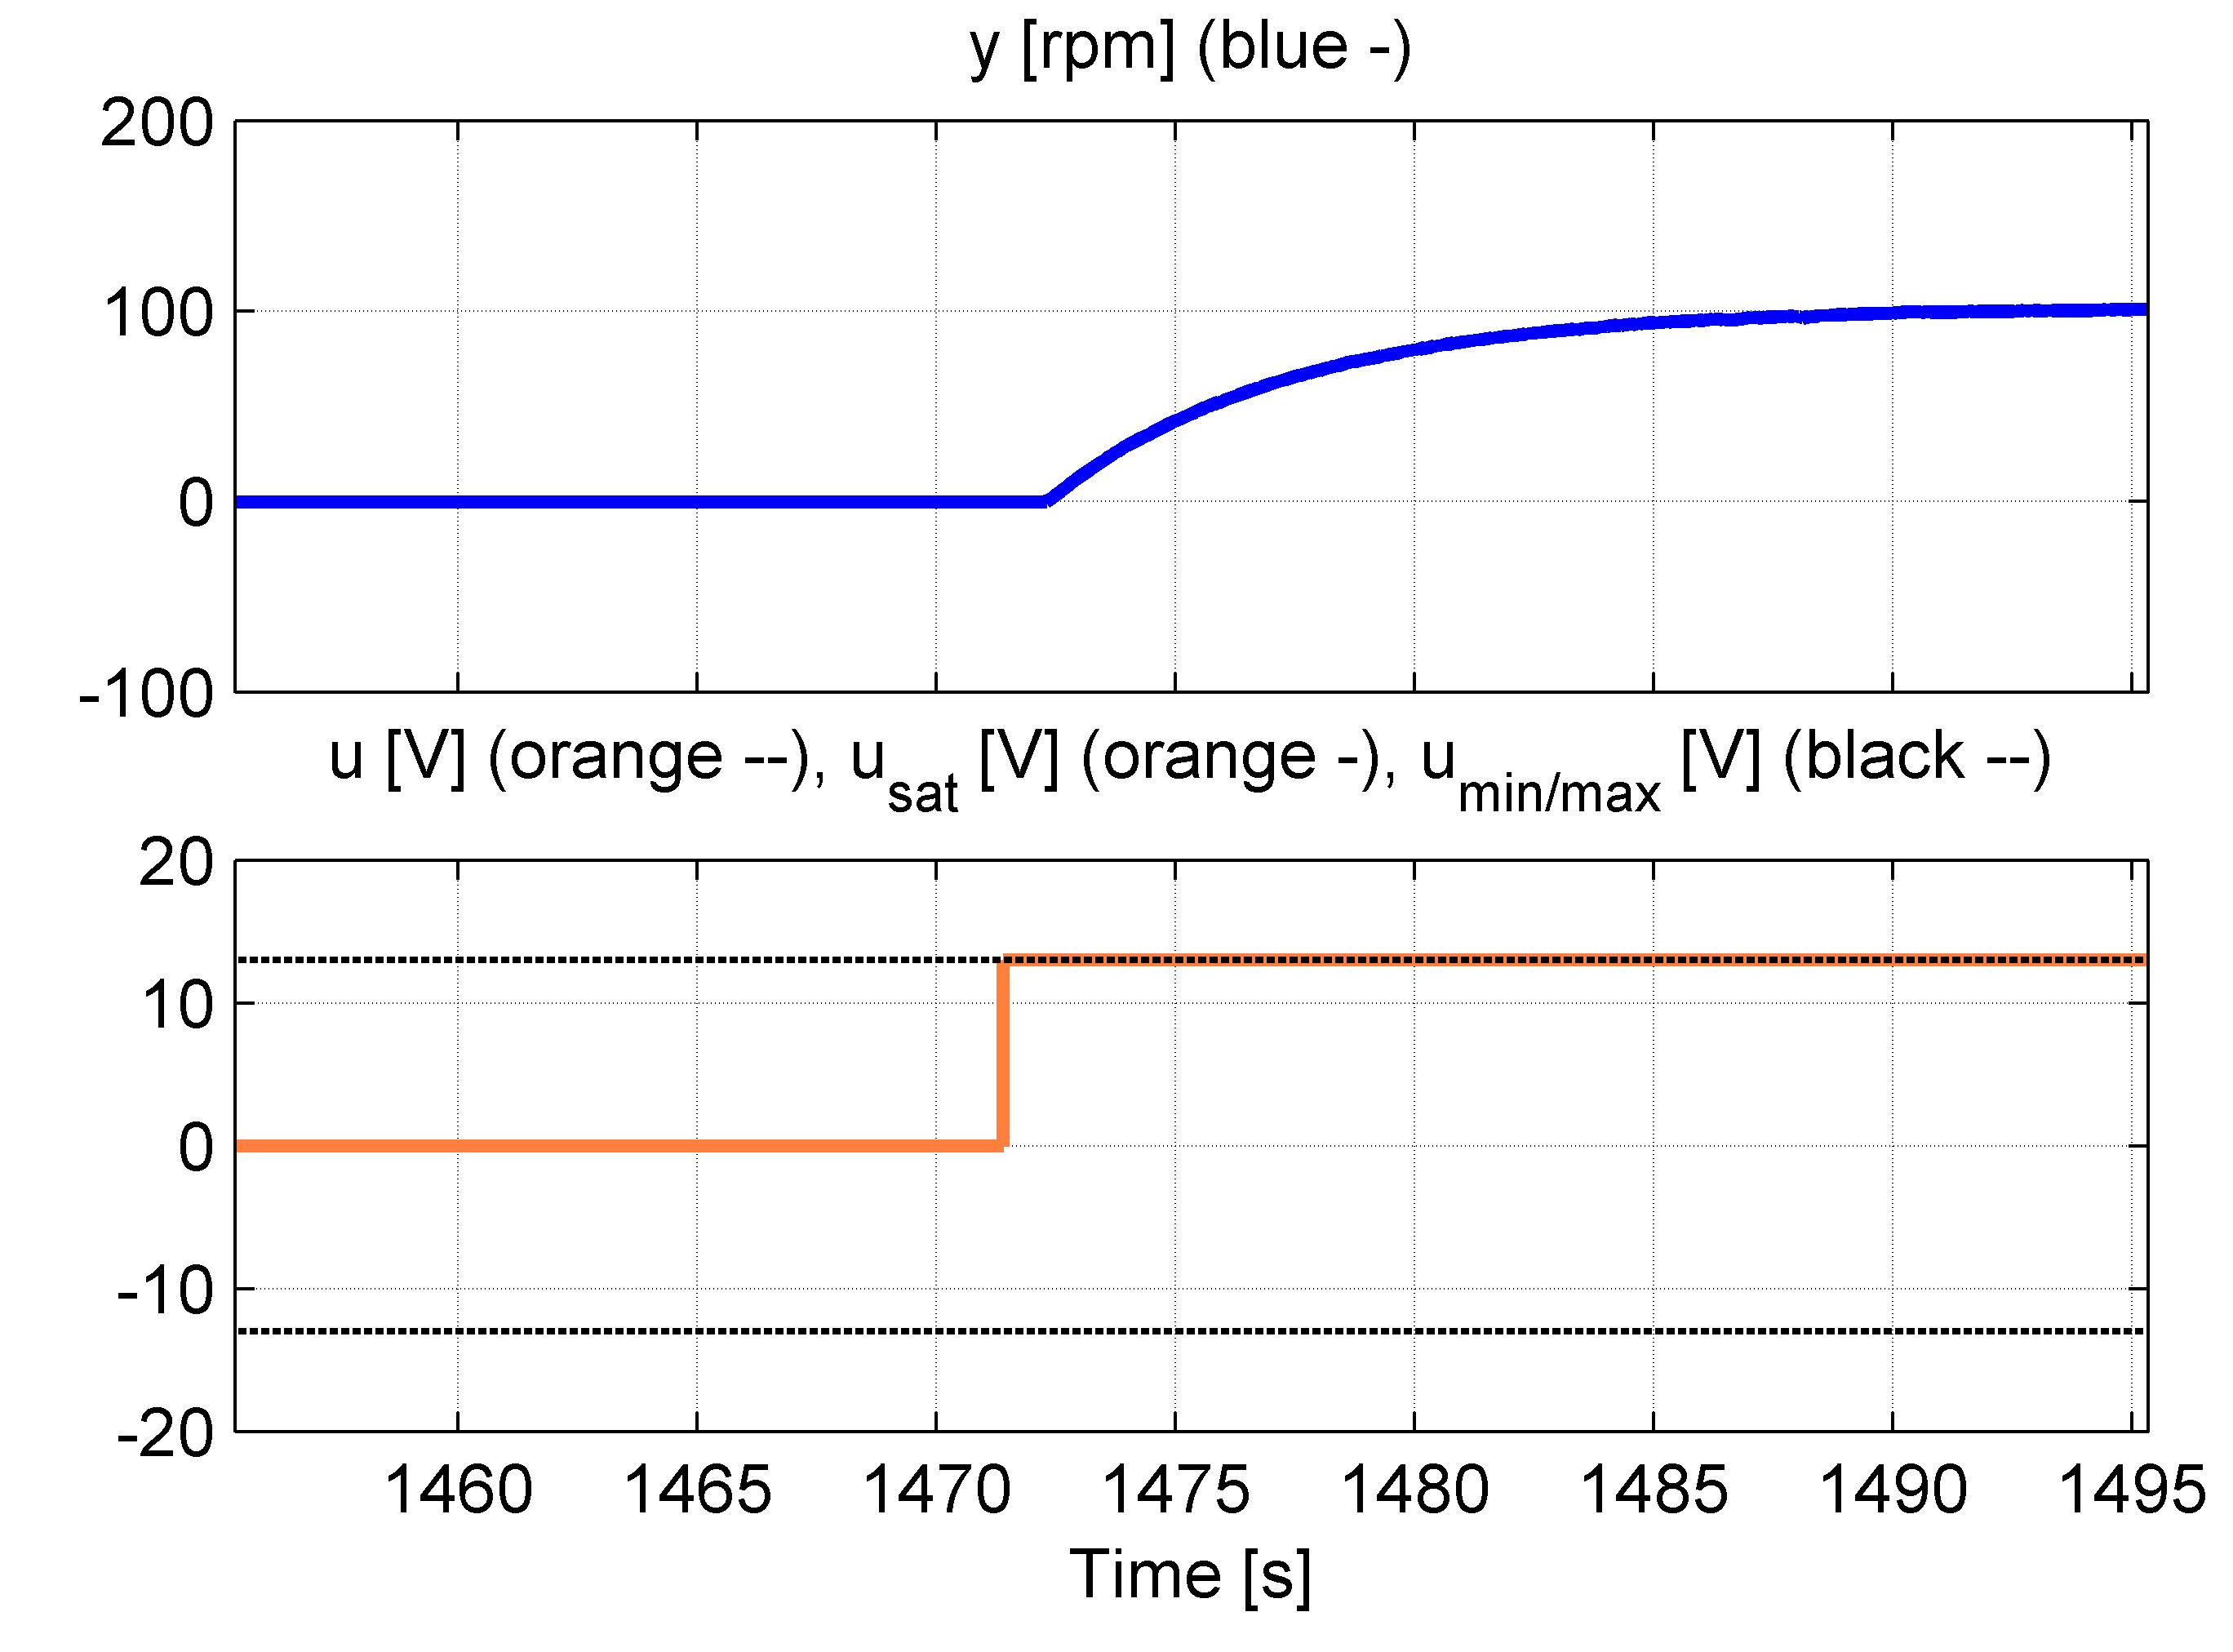
\includegraphics[width=0.6\linewidth]{images/general/Step_Response}
\end{center}
\caption{Step response of a $PT_2$ element}
\label{fig:Step_Response}
\end{figure}

Using the turn tangent principle depicted in Figure \ref{fig:wendetangentenverfahren}, the parameters $T_u$, $T_g$ and $K_s$ were derived.

\begin{figure}[H]
\begin{center}
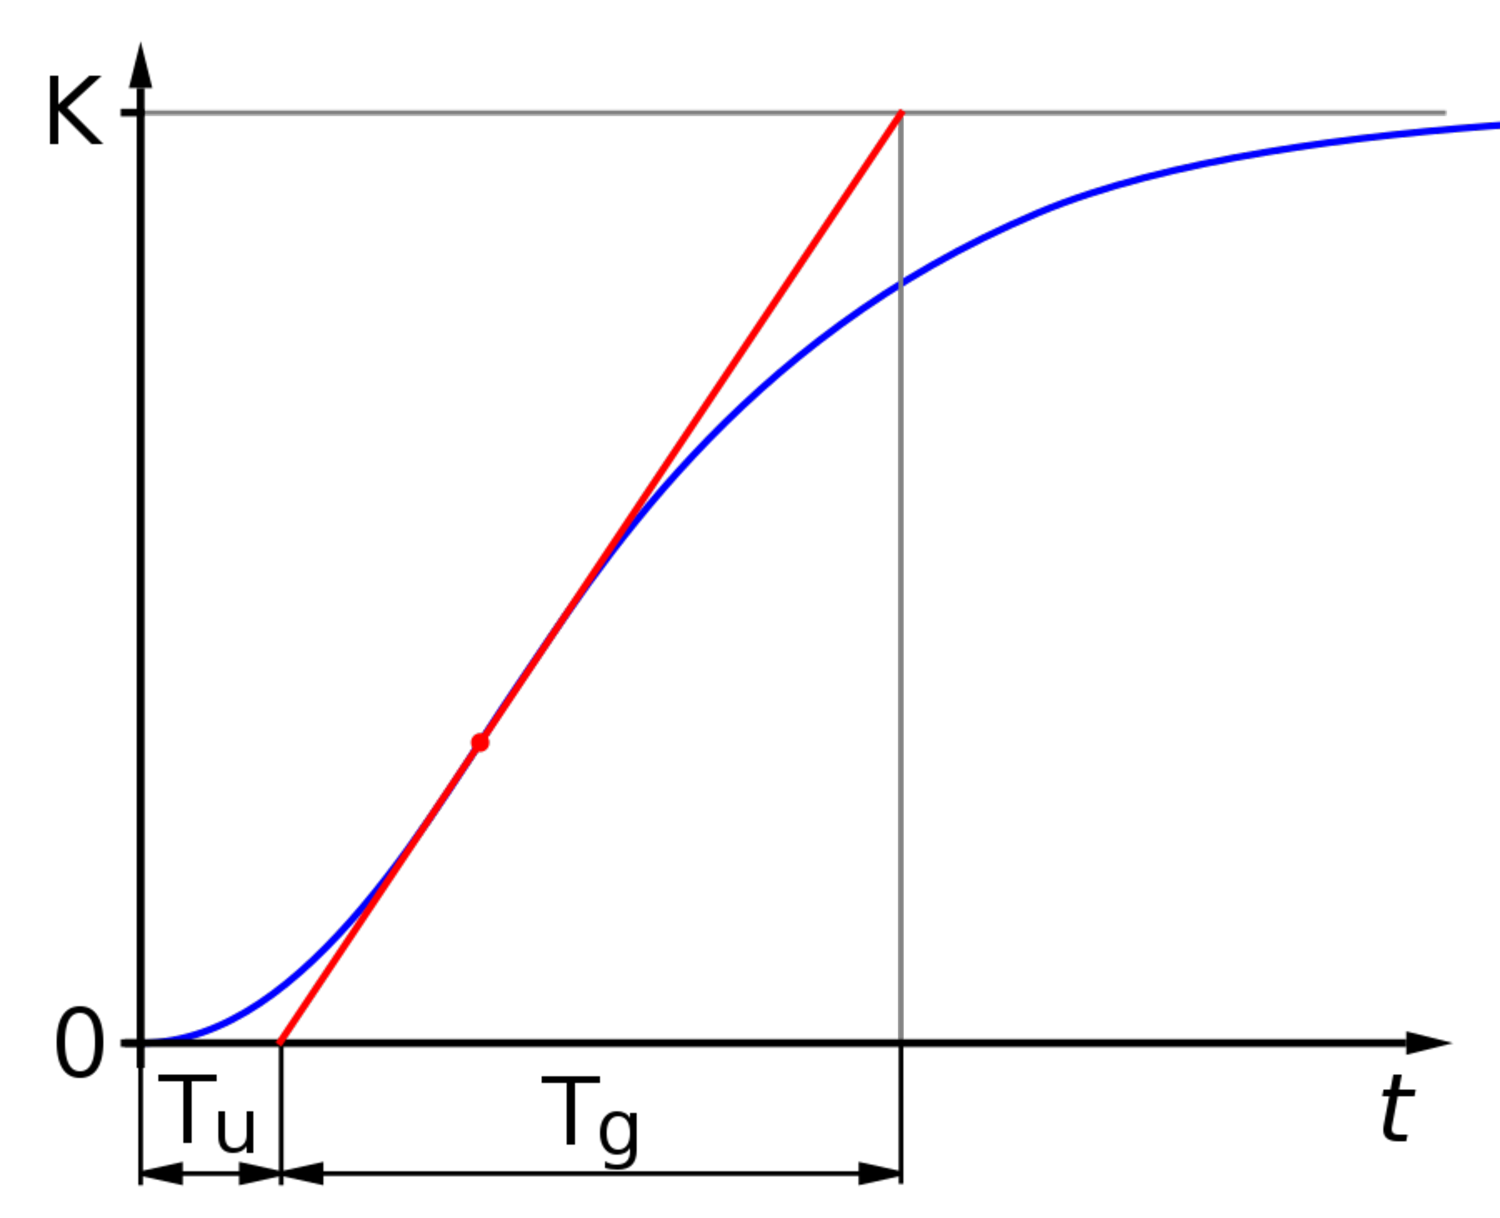
\includegraphics[width=0.6\linewidth]{images/general/wendetangentenverfahren}
\end{center}
\caption{Step response of a $PT_2$ element}
\label{fig:wendetangentenverfahren}
\end{figure}

\begin{center}
\begin{tabular}{ |c|c| } 
 \hline
 Parameters & Values \\ \hline
 $T_{u}(sec)$ & 1   \\  
 \hline
 $T_{g}(sec)$ & 2  \\ \hline
 $K_{s}$ & 10 \\ \hline
\end{tabular}
\end{center}


\subsection{Oscillation Experiment}
The figure below is the oscillation experiment out of which the critical gain and critical period were determined.
\begin{figure}[H]
\begin{center}
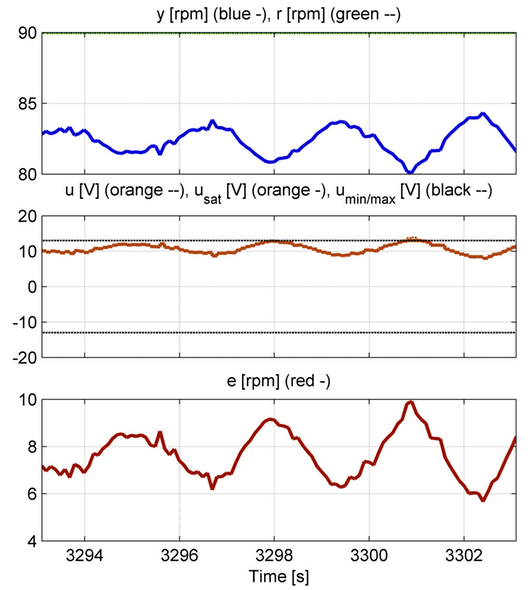
\includegraphics[width=0.6\linewidth]{images/general/Oscillation_Experiment}
\end{center}
\caption{Critical gain $K_{P,crit}$ and $\tau_{crit} $}
\label{fig:Oscillation_Experiment}
\end{figure}
\section{Evaluation}
\section{Control Design}

For the three types of controllers,different characteristic parameters are used. The procedure was carried on with various setpoints which portrayed the operating points. The graphs part show the different experiments:
\subsection{P-Controller}
The P-Controllers with the different parameters are illustrated graphically as follows: \textbf{$K_{P,rule}$} $= 0.7$
\subsubsection{P-Controller}
In the experiment of the P-controller shows that the deviation of the error decreases with the increasing of $K_{p}$.
\begin{center}
{$K_{p}= K_{P,rule}\cdot{0.2}$}
\end{center}

\begin{figure}[H]
\begin{center}
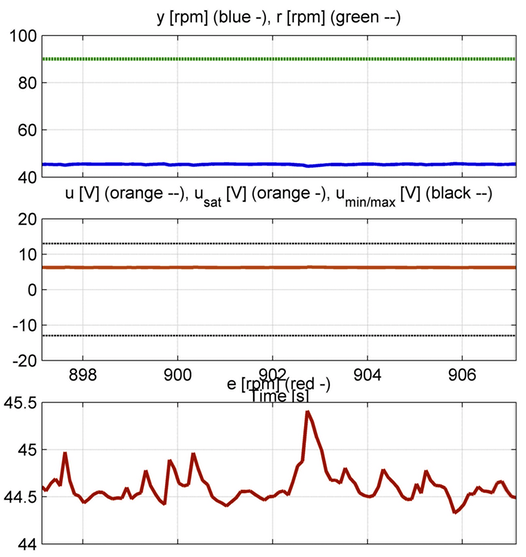
\includegraphics[width=0.6\linewidth]{images/general/P/p_controller02}
\end{center}
\caption{P-Controller of $ K_{P,rule}*\cdot{0.2}$}
\label{fig:p_controller2}
\end{figure}

\begin{center}
{$K_{p}= K_{P,rule}$}
\end{center}
\begin{figure}[H]
\begin{center}
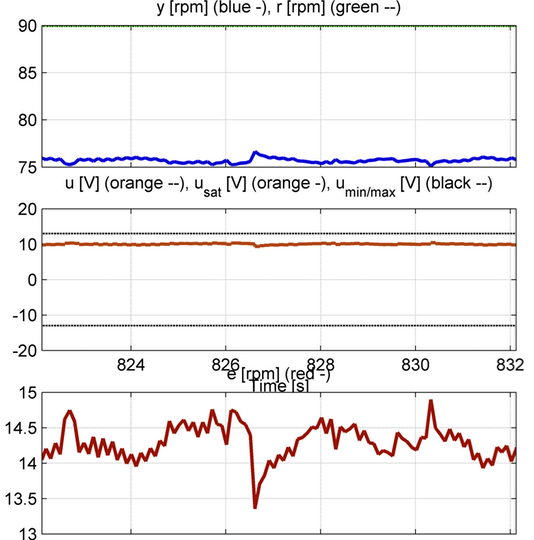
\includegraphics[width=0.6\linewidth]{images/general//P/p_controller1}
\end{center}
\caption{P-Controller of $ K_{P,rule}$}
\label{fig:p_controller1}
\end{figure}

\begin{center}
{$K_{p}= K_{P,rule}\cdot4$}
\end{center}
\begin{figure}[H]
\begin{center}
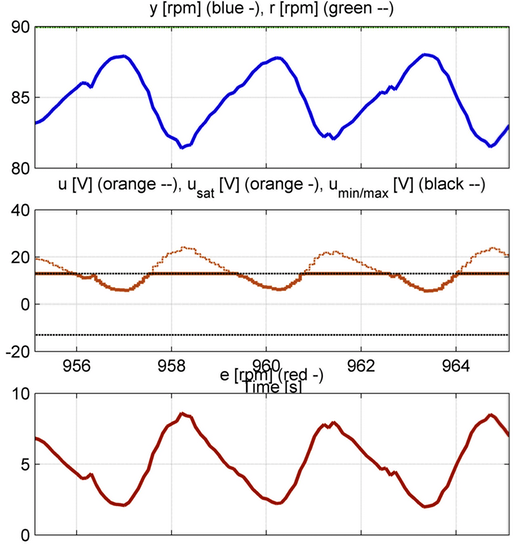
\includegraphics[width=0.6\linewidth]{images/general//P/p_controller4}
\end{center}
\caption{P-Controller of $ T_{T,rule}\cdot{4}$}
\label{fig:p_controller4}
\end{figure}
\clearpage

\subsection{PI-Controller}
In this experiment, the increase of $ T_{i}$ reduces the overshoot  which slows to reach the setpoint whereas the decrease of $ T_{i}$ generates high oscillation with fast rise time that forces the controller to reach the setpoint in short time.
\begin{center}
{$K_{p}= K_{P,rule}$ and $ T_{i,rule}\cdot0.2$}
\end{center} 
\begin{figure}[H]
\begin{center}
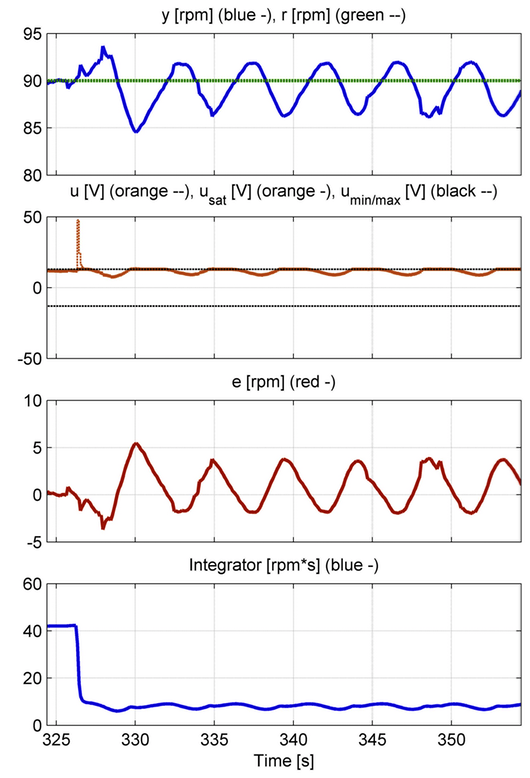
\includegraphics[width=0.6\linewidth]{images/general//PI/PI_Controller02}
\end{center}
\caption{P-Controller of $ T_{i,rule}\cdot{0.2}$}
\label{fig:PI_Controller02}
\end{figure}

The figure below is for the Rise time of the PI-Controller with parameter $T_{i}=0.2\cdot{T_{i,rule}}$.
\begin{figure}[H]
\begin{center}
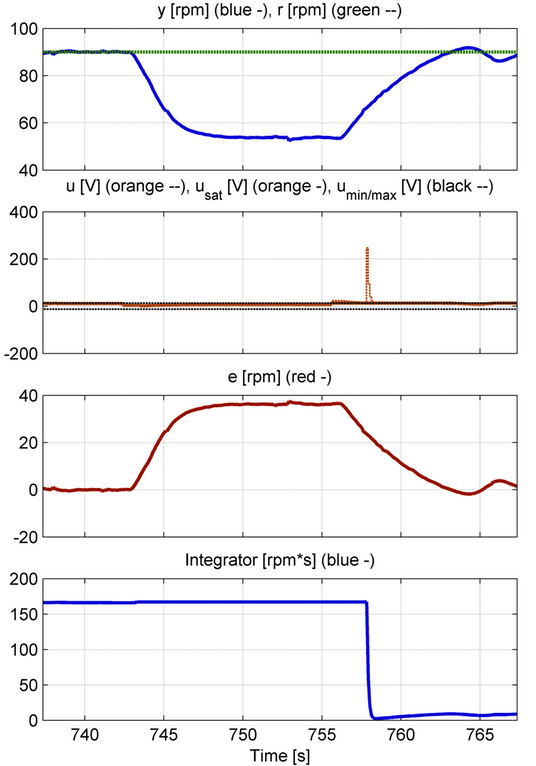
\includegraphics[width=0.6\linewidth]{images/general//PI/PI_RiseTime02}
\end{center}
\caption{P-Controller of $ T_{I,rule}\cdot{0.2}$}
\label{fig:PI_RiseTime02}
\end{figure}

\begin{center}
{$K_{p}= K_{p,rule}$ and $T_{i}=T_{i,rule}$}
\end{center}
\begin{figure}[H]
\begin{center}
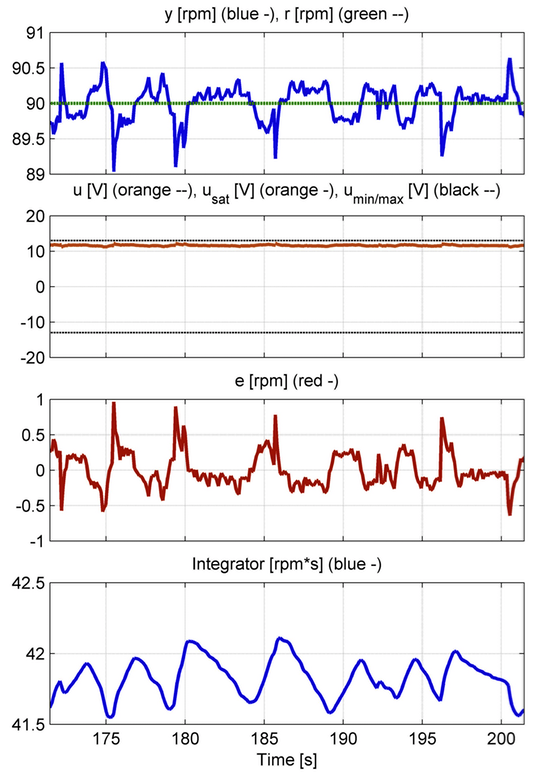
\includegraphics[width=0.6\linewidth]{images/general//PI/PI_Controller1}
\end{center}
\caption{P-Controller of $ T_{i,rule}$}
\label{fig:PI_Controller02}
\end{figure}
The figure below is for the Rise time of the PI-Controller with parameter $T_{i}= {T_{i,rule}}$
\begin{figure}[H]
\begin{center}
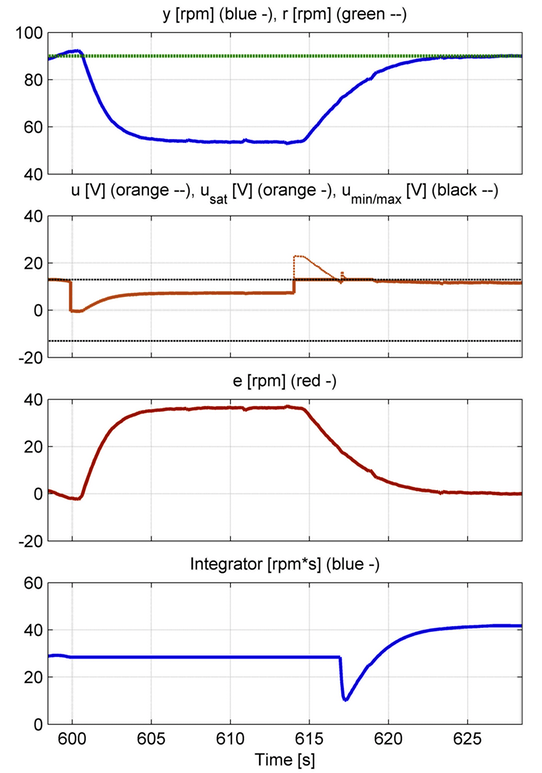
\includegraphics[width=0.6\linewidth]{images/general//PI/PI_RiseTime1}
\end{center}
\caption{P-Controller of $ T_{i,rule}$}
\label{fig:PI_RiseTime1}
\end{figure}

\begin{center}
{$K_{p}= K_{P,rule}$ and $T_{i}=T_{i,rule}\cdot4$}
\end{center}
\begin{figure}[H]
\begin{center}
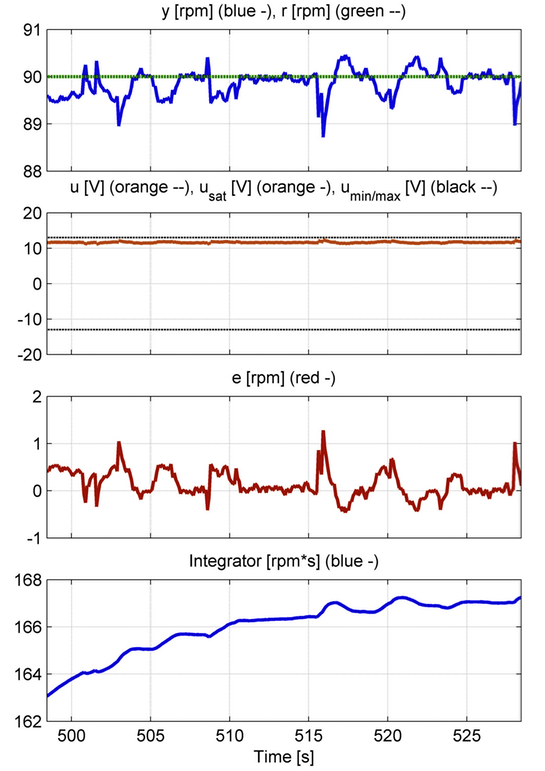
\includegraphics[width=0.6\linewidth]{images/general//PI/PI_Controller4}
\end{center}
\caption{P-Controller of $ K_{P,rule}\cdot4$}
\label{fig:PI_Controller4}
\end{figure}

The figure below is for the Rise time of the PI-Controller with parameter $T_{i}=4\cdot{T_{i,rule}}$
\begin{figure}[H]
\begin{center}
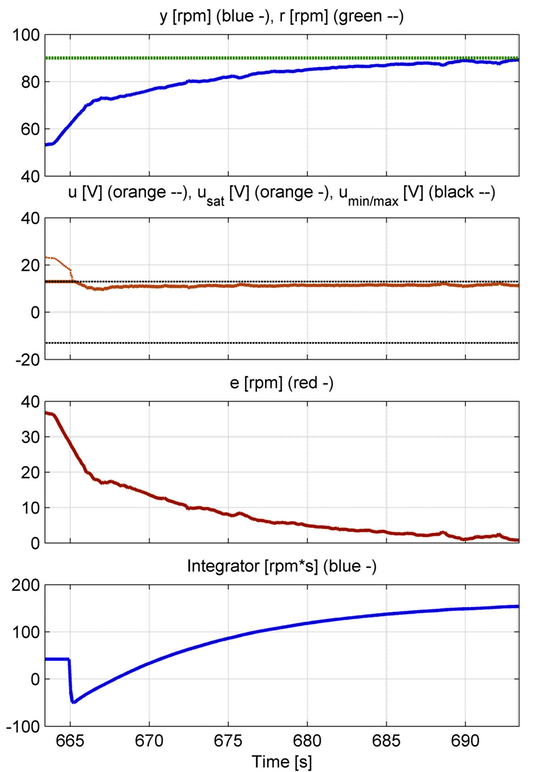
\includegraphics[width=0.6\linewidth]{images/general//PI/PI_RiseTime4}
\end{center}
\caption{P-Controller of $ K_{P,rule}\cdot4$}
\label{fig:PI_RiseTime4}
\end{figure}
\clearpage
\subsection{PID-Controller}
The Ziegler-Nichols and Chien-Hrones-Reswick methods of tuning PID controllers have been used for the following part of the experiment. The depiction shows clearly that the Chien-Hrones-Reswick is a lot faster than Ziegler-Nichols method.
\begin{center}
\begin{tabular}{ |c|c| } 
 \hline
 Parameters & Values \\ \hline
 $T_{d}(sec)$ & 0.32   \\  
 \hline
 $T_{i}(sec)$ & 1.33  \\ \hline
 $K_{p}$ & 0.84 \\ \hline
\end{tabular}
\end{center}

\begin{figure}[H]
\begin{center}
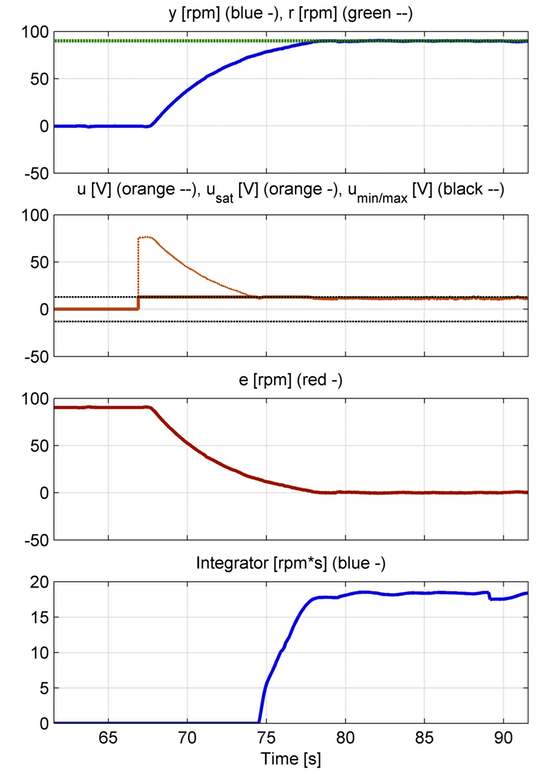
\includegraphics[width=0.6\linewidth]{images/general//PID/Ziegler_nichols}
\end{center}
\caption{  Chien-Hrones-Reswick tuning rule for $T_{i}, T_{d},K_{P}$ }
\label{fig:Ziegler_nichols}
\end{figure}


\begin{figure}[H]
\begin{center}
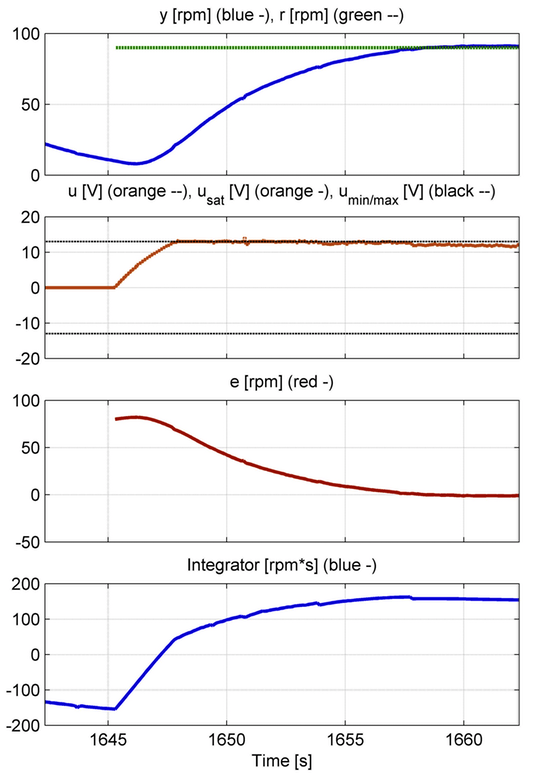
\includegraphics[width=0.6\linewidth]{images/general//PID/Chien_Hrones_Reswick}
\end{center}
\caption{Ziegler-nichols tuning rule for $T_{i}, T_{d},K_{P}$}
\label{fig:Chien_Hrones_Reswick}
\end{figure}